%% 
%% Copyright 2019 Elsevier Ltd
%% 
%%
%%%%%%%%%%%%%%%%%%%%%%%%%%%% ! ! ! SUBMISSION CHECKLIST ! ! ! %%%%%%%%%%%%%%%%%%%%%%%%%%%%
%%
%% Please confirm that your submission follows all the requirements of the guidelines, including the submission checklist:
%% _ Cover letter
%% _ Highlights
%% _ Authorship statement
%% _ The manuscript must be single column and double spaced
%% _ Reference must be in the author-date format
%% _ Code availability section 
%%
%% *All the manuscripts in disagreement with the guidelines will be desk-rejected without editorial check.
%%
%% --------------------------------------
%%
%% This file is part of the 'CAS Bundle'.
%%  
%% It may be distributed under the conditions of the LaTeX Project Public
%% License, either version 1.2 of this license or (at your option) any
%% later version.  The latest version of this license is in 
%%    http://www.latex-project.org/lppl.txt 
%% and version 1.2 or later is part of all distributions of LaTeX
%% version 1999/12/01 or later.
%%   
%% The list of all files belonging to the 'CAS Bundle' is
%% given in the file `manifest.txt'.
%% 
%% Template article for cas-dc documentclass for  
%% double column output.
 
%\documentclass[a4paper,fleqn,longmktitle]{cas-dc}
\documentclass[a4paper,fleqn]{cas-sc}

\usepackage[authoryear]{natbib}
\usepackage{graphicx} 
\usepackage{float}
\usepackage{algorithm}  
\usepackage{algpseudocode}
\usepackage{color}
\usepackage{setspace}
\usepackage[nomarkers,figuresonly]{endfloat}


\newcommand{\colorComments}{black} 
 
%%%Author definitions
\def\tsc#1{\csdef{#1}{\textsc{\lowercase{#1}}\xspace}}
\tsc{WGM}
\tsc{QE}
\tsc{EP}
\tsc{PMS}
\tsc{BEC}
\tsc{DE}
%%%

\usepackage{lineno}
\linenumbers 

\begin{document}
\let\WriteBookmarks\relax
\def\floatpagepagefraction{1}
\def\textpagefraction{.001}
\shorttitle{Short title}
\shortauthors{short author name}

\title [mode = title]{Manuscript title - \LaTeX  template for Computers \& Geosciences  }


\author[1]{Author 1}[type=editor,
                        auid=000,bioid=1,orcid=0000-0000-0000-0000]
\credit{ Author 1 contribution  }

\author[2]{Author 2} 
\credit{Author 2 contribution }

\author[3]{Author 3}
\credit{Author 3 contribution}

\address[1]{Author 1 affiliation}
\address[2]{Author 2 affiliation}
\address[3]{Author 3 affiliation} 

\begin{abstract}
Abstract text here, abstract text here,  abstract text here,  abstract text here,  abstract text here,  abstract text here,  abstract text here,  abstract text here,  abstract text here,  abstract text here,  abstract text here,  abstract text here,  abstract text here,  abstract text here,  abstract text here,  abstract text here,  abstract text here,  abstract text here,  abstract text here.
\end{abstract}

% 注释内容
\iffalse 
\begin{coverletter}

Dear Editors-in-Chief,
\newline
 
please find the enclosed manuscript "..." which we are submitting for exclusive consideration for publication in Computers \& Geosciences. We confirm that the submission follows all the requirements and includes all the items of the submission checklist.  
\newline
 
The manuscript presents ... 
\newline

We provide the source codes in a public repository with details listed in the section "Code availability".
\newline

Thanks for your consideration. 
\newline

Sincerely,
\newline

Authors names

Corresponding author affiliation and e-mail
\newline

\textbf{Delete before submission:}

Please confirm that your submission follows all the requirements of the guidelines, including the submission checklist:

- Cover letter

- Highlights

- Authorship statement

- The manuscript must be single column and double spaced

- Reference must be in the author-date format

- Code availability section 

*The manuscripts that do meet the requirement guidelines will be desk-rejected.



\end{coverletter}

\begin{highlights}
\item Highlight 1
\item Highlight 2
\item Highlight 3
\item Highlight 4
\item Highlight 5
\end{highlights}
\fi


% 正文

\begin{keywords}
Keyword 1 \sep Keyword 2 \sep Keyword 3 \sep Keyword 4
\end{keywords}

\maketitle 

\printcredits

\doublespacing


\section{Introduction}
\label{intro}
With the continuous advancement of unconventional oil and gas exploration and development, the limitations of traditional rock physics methods---such as dependency on laboratory conditions, lengthy experimental cycles, and low data acquisition efficiency---have become increasingly prominent. To enhance the characterization of reservoir microstructures, Digital Rock Physics (DRP), an interdisciplinary technique that integrates image processing, computational modeling, and numerical simulation, has attracted widespread attention in recent years in the fields of rock physics, reservoir characterization, and geotechnical engineering (reference). %(哪些文献表明)

Currently, digital rock modeling primarily relies on image data obtained from micro-computed tomography (Micro-CT) and scanning electron microscopy (SEM). Micro-CT enables non-destructive acquisition of the three-dimensional structure of rock samples, offering good structural connectivity and a relatively large field of view (FoV); however, its spatial resolution is limited, making it insufficient for accurately capturing pore structures at the micrometer or nanometer scale. In contrast, SEM images provide significantly higher resolution and can reveal intricate microstructural features, but the imaging range is limited, typically two-dimensional, and the acquisition process is costly and time-consuming (reference). %(哪些文献表明)

In digital image-based modeling, FoV and image resolution are two key but inherently constrained parameters. Due to current limitations in imaging technology, there exists an intrinsic trade-off between FoV and resolution: enhancing spatial resolution often results in a reduced observable area, while expanding the FoV generally leads to lower resolution (reference). %(哪些文献表明) This trade-off restricts the ability to build high-quality image-based models at a unified scale, particularly when both macroscopic structural integrity and microscopic detail preservation are required.

\section{Related Work}

\subsection{Digital Rock Physics and Imaging Modalities}

\subsection{GAN-Based Approaches for Multiscale Image Generation}

\subsection{Framework and Architectural Innovations}

\section{Method}


\subsection{Overview of CycleGAN generation framework}

CycleGAN is used as the basic frame to realize the cross-domain transformation between unpaired images. CycleGAN is an unsupervised image-to-image translation model first proposed by Zhu et al. in 2017. This method is a method for unsupervised image conversion between two image domains X and Y.The goal is to learn the mapping function in two directions without paired samples:$G:X \rightarrow Y$ and$F:Y \rightarrow X$ ,where the training data comes from source domain samples $\{x_i\}_{i=1}^N$and target domain sample$\{y_j\}_{i=1}^N$, and respectively obeys the distribution$x \sim p_{data}(x)$ and $y \sim p_{data}(y)$

% todo 新增图1
As shown in Figure 1, the CycleGAN network includes two generators $G$ and $F$, and two discriminators $D_Y$ and $D_X$. Among them, the discriminator $D_Y$ is used to determine whether the image $y$ and the generated image $G(x)$ come from the same distribution; similarly, the discriminator $D_X$ aims to distinguish the real source domain image $x$ from the reconstructed image $F(y)$.

In CycleGAN, the optimization goal consists of two core loss terms: Adversarial Loss and Cycle Consistency Loss, which together act on the modeling process of unsupervised image-to-image conversion.

(1)\textbf{Adversarial Loss}

Combating loss is used to ensure that the distribution of the generated image is as close as possible to the data distribution in the target domain. Specifically, for the mapping $G:X \rightarrow Y$ from the source domain $X$ to the target domain $Y$, CycleGAN introduces a discriminator $D_Y$ to distinguish between the real image y and the generated image $G(x)$, such that:

\begin{equation}
	\mathcal{L}_{GAN}(G, D_Y, X, Y) = \mathbb{E}_{y \sim p_{data}(y)}[\log D_Y(y)] + \mathbb{E}_{x \sim p_{data}(x)}[\log(1 - D_Y(G(x)))]
\end{equation}


Similarly, for the inverse mapping $F:Y \rightarrow X$, a discriminator $D_X$ is introduced to distinguish the real source image $x$ from the synthetic image $F(y)$, forming another antagonistic loss term.
Such losses drive the generator to learn realistic mapping results, but do not by themselves ensure a one-to-one semantic or structural relationship between inputs and outputs.


(2)\textbf{cycle consistency loss}
In order to avoid pattern crashes or non-semantic alignment problems caused by adversarial training alone, CycleGAN proposes cyclic consistency constraints. The core idea is: After mapping once and then mapping back, the original image should be restored as much as possible, that is:

\begin{itemize}
	\item forward consistency:$x \rightarrow G(x) \rightarrow F(G(x)) \approx x$
	\item Reverse consistency:$y \rightarrow F(y) \rightarrow G(F(y)) \approx y$
\end{itemize}

The cyclic consistency loss function is defined as:
\begin{equation}
	\mathcal{L}_{cyc}(G, F) = \mathbb{E}_{x \sim p_{data}(x)}[\|F(G(x)) - x\|_1] + \mathbb{E}_{y \sim p_{data}(y)}[\|G(F(y)) - y\|_1]
\end{equation}

The loss term measures the difference between the restored image and the original image through the L1 norm, effectively constraining the mapping result to maintain structural and semantic consistency.

(3)\textbf{total loss function}
Finally, CycleGAN's total loss function integrates the two loss forms as follows: 
\begin{equation}
	\mathcal{L}(G, F, D_X, D_Y) = \mathcal{L}_{GAN}(G, D_Y, X, Y) + \mathcal{L}_{GAN}(F, D_X, Y, X) + \lambda \mathcal{L}_{cyc}(G, F)
\end{equation}
Among them, the hyperparameter $\lambda$ controls the weight of the loop consistency loss in the overall objective function
\subsection{Modified CycleGAN for Micro-CT to SEM Translation}

Although the basic CycleGAN framework performs well in unsupervised image domain conversion tasks, there are still the following challenges in the high-resolution conversion task of Micro-CT images to SEM images: on the one hand, structural information in Micro-CT images is relatively fuzzy, and direct mapping often leads to the generated image lacking sufficient texture detail and boundary sharpness; on the other hand, SEM images have richer high-frequency textures and microscopic pore structures, which puts higher requirements on the generator's modeling capabilities.


To this end, this paper introduces a number of structural improvements based on the traditional CycleGAN architecture to improve the model's performance in detail restoration and image quality, mainly including:

1.Introduce a multi-scale feature fusion module into the generator to enhance the perception of pore structures of different size;

2.Use the multi-scale PatchGAN discriminator to jointly discriminate local and global textures to guide the generated images to maintain semantic consistency in multi-level spaces;

3.Optimize the up-sampling module and use interpolation fusion and residual connection to effectively alleviate the edge ambiguity problem in the up-sampling process;

4.In terms of loss function, in addition to retaining the original confrontation loss and cyclic consistency loss, structure preservation loss and edge enhancement terms are also added to further enhance the ability to model microstructure and boundary information.

Through the above improvements, the model can better capture the differences in spatial frequency, structural details and texture distribution between Micro-CT images and SEM images, thereby generating high-resolution rock images that are more realistic and scientifically explanatory. 

\subsubsection{multi-scale discriminator}

\subsection{Data and Training Settings}


\begin{equation}
\label{eqn:linear}
    y=ax+b.
\end{equation}


\begin{equation} 
\label{eqn:quadratic}
    y=ax^2+bx+c
\end{equation}

\section{Algorithm and implementation}

Example of algorithm:
\begin{algorithm}
  \caption{Algorithm example }
  
  \begin{algorithmic}
  \label{alg:Alg1}
  \State \textbf{Input:} ...
   \newline

 \Statex \textit{1.} Step1
  \Statex \textit{2.} Step2;
 \State \textit{3.}  Step3;
  \newline
   \For{ i = 1,..., m}
   \State \textit{4.} Step 4;
    \For{ j = 2,..., n} 
   \State \textit{5.}  Step 5;
   \State \textit{6.} Step 6;
   \EndFor
  \EndFor 
  \newline
\State  \textbf{Output: } ... 
  \end{algorithmic} 
\end{algorithm} 


\section{Results}


This section includes an example of figure (Figure \ref{fig:Figure1}), from  \cite{de2021direct}.

\begin{figure}
\centering
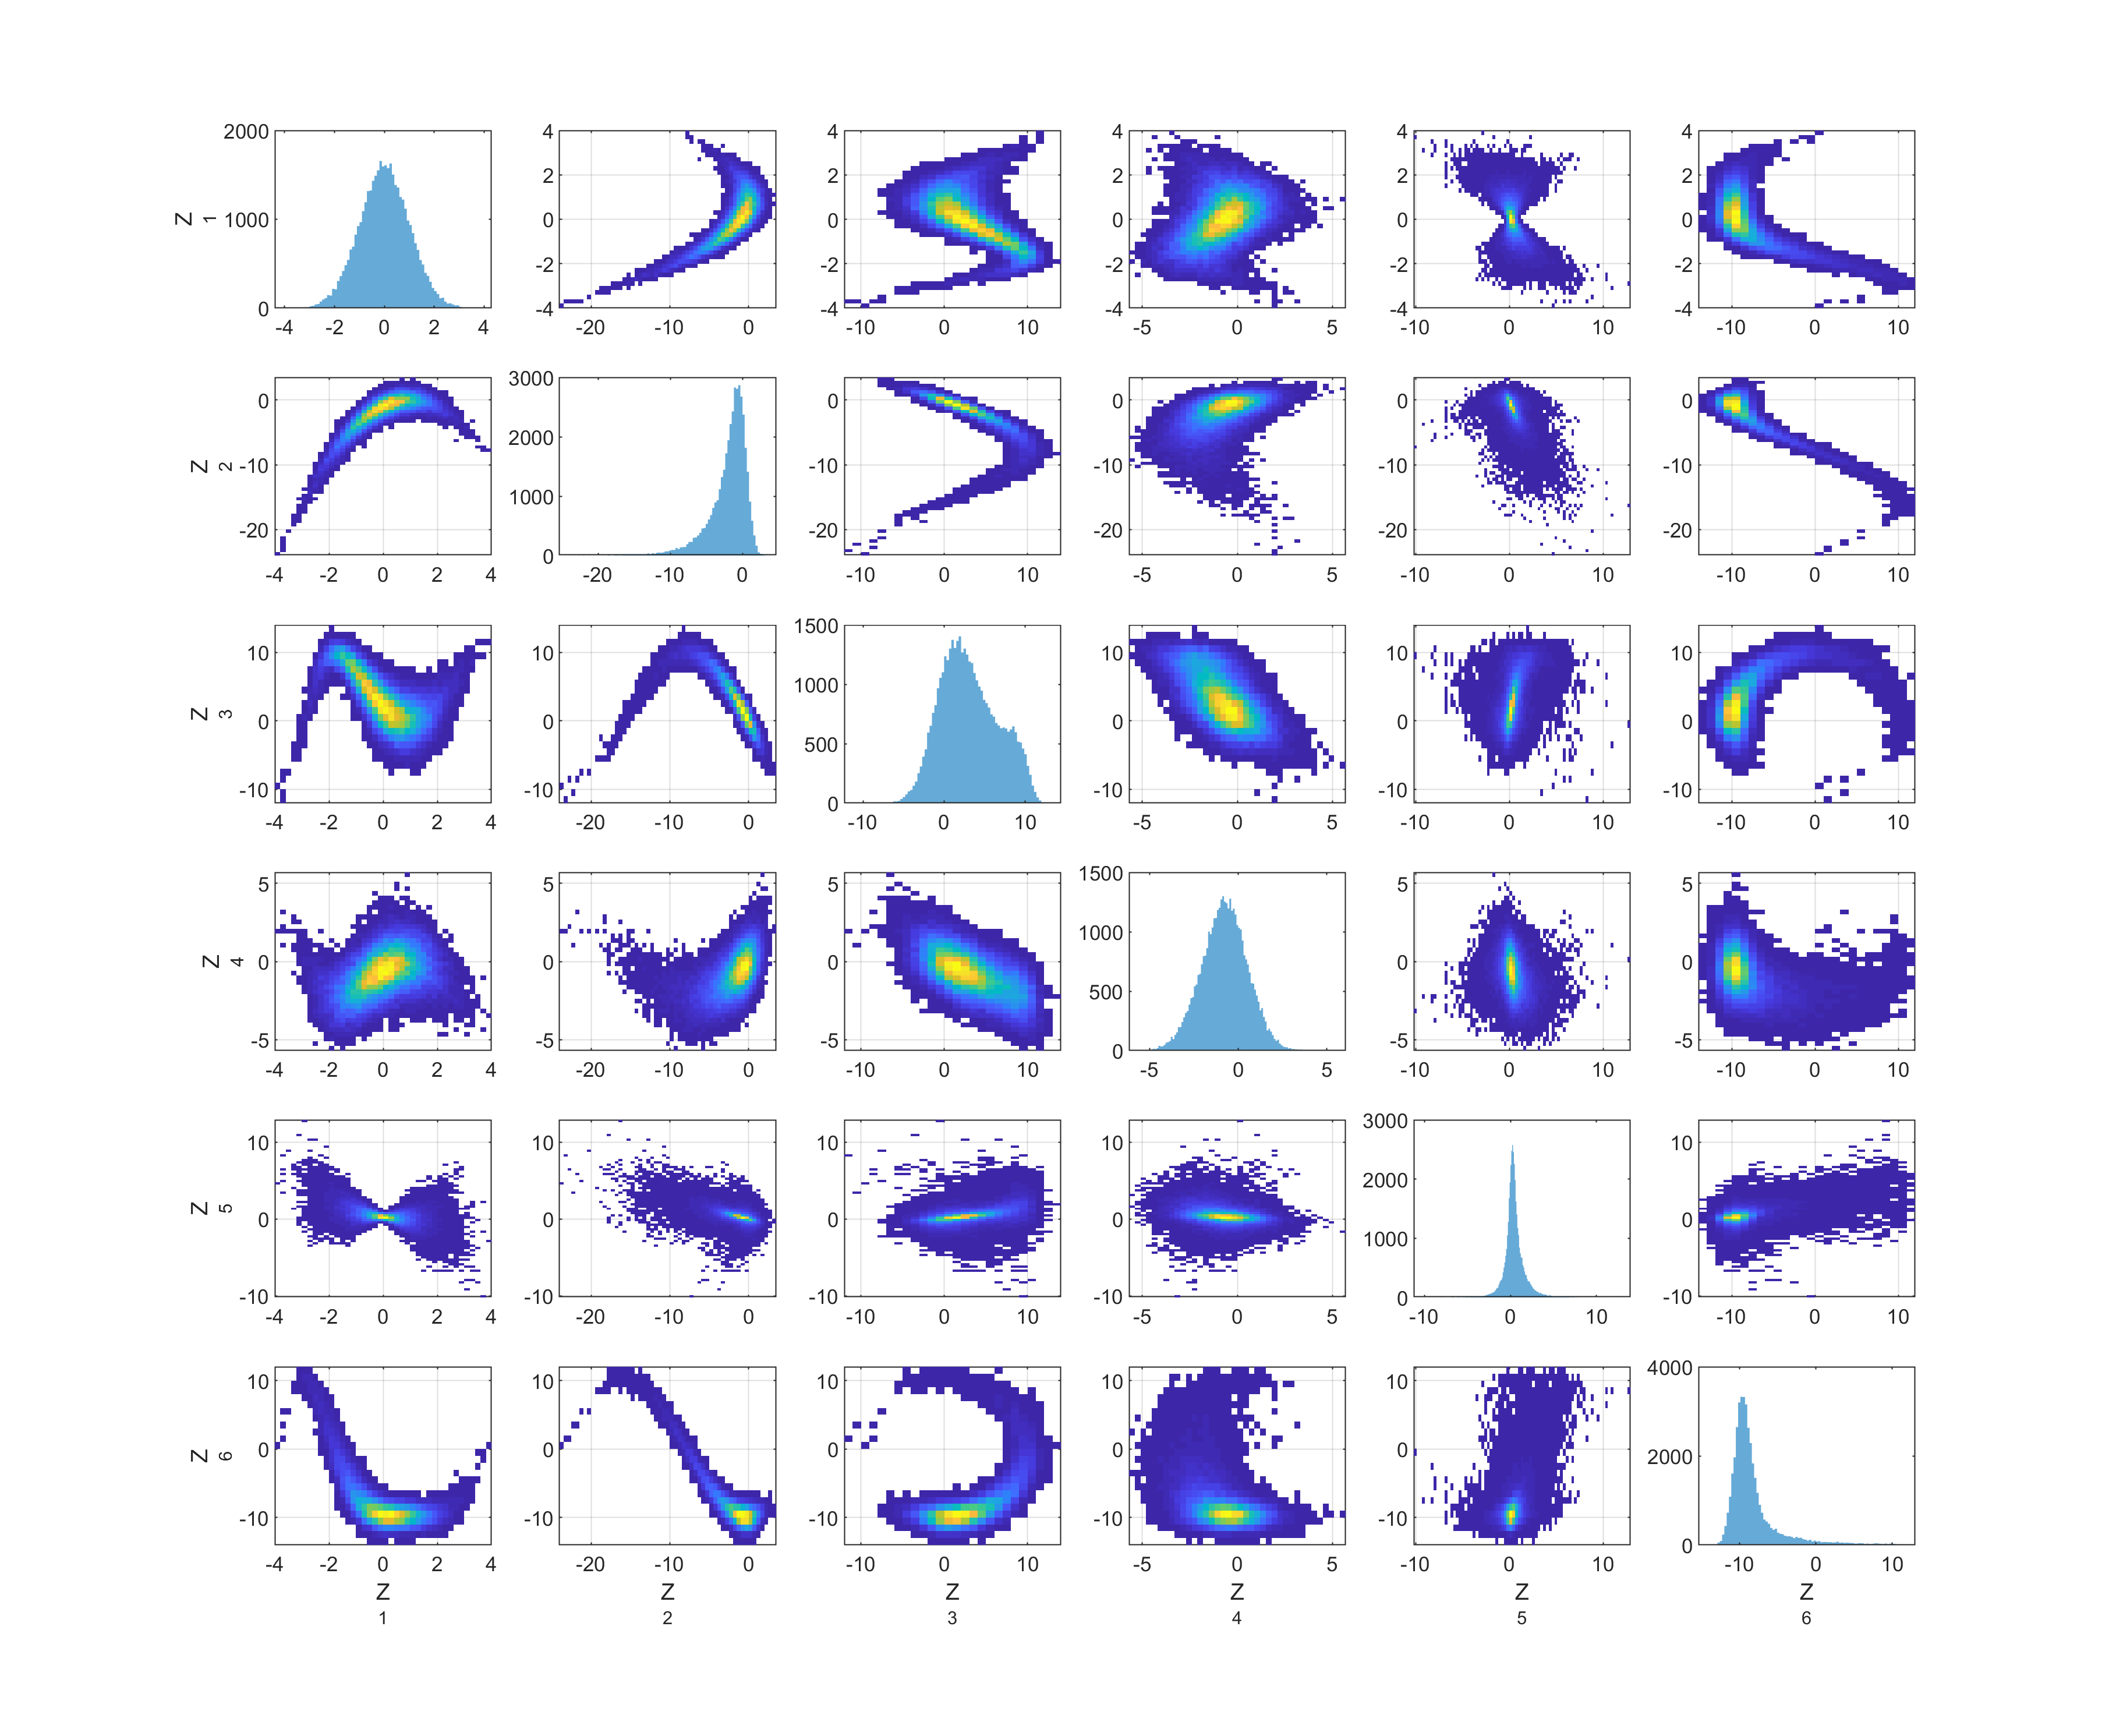
\includegraphics[width=0.75\textwidth]{figs_rev1/uncond_distribution_reference.png}
\caption{ Caption here. Image from \cite{de2021direct}.}
\label{fig:Figure1}
\end{figure}

This section includes an example of table (Table \ref{tab:Table1}).

\begin{table}
\centering
\caption{Example of table.}
\label{tab:Table1}
\begin{tabular}{ |c||c|c|c|} 
 \hline
     & $a$  &  $b$  &  $c$\\ 
 \hline 
 \hline
$a$ & 0.014 &  0.20    &   0.13  \\
\hline
$b$ & 0.20    &   0.17    &   2.46    \\
\hline
$c$ & 0.13    &   2.5     &   0.31   \\
\hline
\end{tabular} 
\end{table}


\subsection{Subsection}

Text ...

\section{Conclusions}

Conclusions here...

\section{Acknowledgments}

The authors would like to acknowledge ...

\newpage

\textbf{Code availability section}

Name of the code/library

Contact: e-mail and phone number

Hardware requirements: ...

Program language: ...
 
Software required: ...

Program size: ...

The source codes are available for downloading at the link:
https://github.com/ . . . . 


\bibliographystyle{cas-model2-names}
\bibliography{bibliography} 

\end{document}

